\documentclass[hyperref,xspace]{beamer}

\usepackage{xspace}
\usepackage{tabularx}
\usepackage{calc}
\usepackage{rotating}
\usepackage{alltt}
\usepackage{beamerthemeCopenhagen}
\setbeamertemplate{footline}{}

\author{Bob Fuhrer \& Jurgen Vinju}
\title{A Program Analysis Infrastructure for IMP}
\subtitle{(a sketch of one)}
\institute{IBM, Hawthorne}
\date{March 5th, 2007}

\newcommand{\jframe}[3]{\section{#1}\subsection{#2}\frame{\frametitle{#2} #3}}
\newcommand{\jsframe}[2]{\subsection{#1}\frame{\frametitle{#1} #2}}
\newcommand{\sframe}[2]{\frame{\frametitle{#1} #2}}
\renewcommand{\emph}[1]{{\color{red} #1}}

\begin{document}
\maketitle

\jframe{Introduction}{Overview}{
 \setcounter{tocdepth}{1}
 \tableofcontents
 \emph{This is all ongoing and future work}
}

\jsframe{Source code analysis in IDE's}{
\begin{itemize}
 \item Integrated Development Environments (IDE's):
 \begin{itemize}
  \item help understanding code.
  \item help manipulating code.
 \end{itemize}
 \item That's why IDE's contain many \emph{analyses};
 \begin{itemize}
 \item ``Simple'' --- like parsing and name resolution.
 \item ``Advanced'' --- like call graphs and data dependencies.
 \item ``Hairy'' --- like dead code analysis and clone detection.
 \item Static, dynamic, and hybrid
 \item Cross programming language/formalism (Makefiles, Ant, CVS)
 \end{itemize}
 \item Analysis results are  used implicitly in the IDE:
 \begin{itemize}
 \item Code search, Outlining, many forms of hyperlinking, pre-conditions of refactorings,
       source metrics, etc.
 \end{itemize}
\end{itemize}
}

\jsframe{IDE Meta-tooling Platform (IMP)}{
\begin{itemize}
 \item Help the IDE builder by providing framework infra-structure and code generators.
 \item What about source code analysis?
 \item The goal is to help the IDE builder to:
 \begin{itemize}
    \item add analyses to an Eclipse-based IDE for \emph{any} language.
    \item analyze the code using different kinds of analysis methods  
    \item focus on the analysis itself, and not the boilerplate of integration.
    \item express analyses in DSL's as well as directly in Java.
 \end{itemize}
 \item Requirements: fast, small, composable, decoupled
\end{itemize}
}

\jsframe{Experience with The Meta-Environment}{
\begin{itemize}
 \item An environment for constructing IDE's and meta programs
 \item ASF+SDF: extraction of facts and transformation
 \item RScript: relational calculus on facts
 \item RStores: common data-structure for fact representation
 \item Fact browser: pluggable visualization framework
 \item Applied and tested in an academic environment:
 \begin{itemize}
  \item Java dead code detection (static and dynamic analysis)
  \item C comment vs. code consistency checker
  \item C call graph extraction, data dependencies
  \item Grammar analyses for SDF
  \item Connected 3 different kinds of viz. toolkits
  \item Connected 2 different kinds of extracting front-ends
 \end{itemize}
 \item Issues: size, speed and limited visibility.
\end{itemize}

}

\jframe{Vocabulary and Architecture}{Source code representations}{
\begin{center}
\resizebox{.8\textwidth}{!}{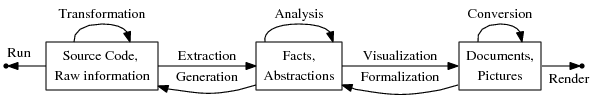
\includegraphics{artefacts.png}}
\end{center}
\begin{enumerate}
 \item ``Extract'' basic undeniable facts from source code
 \item ``Analyze'' the facts and elaborate on them
 \item ``Visualize'' the resulting data in the IDE
\end{enumerate}
}

\jsframe{Architecture and design}{
\begin{center}
\resizebox{.8\textwidth}{!}{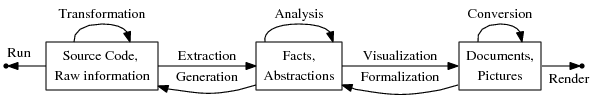
\includegraphics{artefacts.png}}
\end{center}
\begin{itemize}
 \item \emph{Typed relations} are the central data-structure
 \item \emph{Fact Generators} produce facts and store them in the \emph{Fact Base}
 \item \emph{Fact Generators} may also consume facts from the \emph{Fact Base}
 \item \emph{Visualizations} consume facts from the \emph{Fact Base}
 \item Loosely coupled, the \emph{Fact Base} hides by who, how and when a fact is produced.
\end{itemize}
}

\jsframe{A nice picture}{
This page contains our overview picture
}

\jsframe{Type system for relations}{
\begin{itemize}
 \item Goal 1: prevent/diagnose common programming and composition errors.
 \item Goal 2: allow automated discovery and composition of analyses and visualizations.
 \item A simple first-order type system for relations, sets, maps, and atomic values.
 \item Sub-typing with covariance ($ t_1 < t_2 \Rightarrow {set}[t1] < {set}[t2]$)
 \item Mantra: maximize flexibility (reuse), without loosing safety.
\end{itemize}
}

\jframe{High level specification}{}{
\begin{itemize}
 \item DSL's for analysis (and transformation)
 \item Compile down to Java that uses the FactBase and the Relations
 \item DSL's share the type system of relations
 \item Current project: Relational Calculus/Algebraic Data Types
 \begin{itemize}
  \item Operators on sets and relations; comprehensions; fixed point operators
  \item Typed term constructors and normalizing rewrite rules
 \end{itemize} 
\end{itemize}
}

\jsframe{Example --- Infer generic type arguments}{
\begin{itemize}
 \item Problem: transform to Java code that uses generics
 \begin{itemize}
   \item The current Java program represents a set of constraints on the types of variables
   \item First find these constraints using Java static semantics
   \item Then find least general type parameters for variables, satisfying the constraints
 \end{itemize}
 \item The type universe is \emph{very} big
 \item While solving the constraint system, intermediate results (sets of types) can not be kept in main memory
\end{itemize}
}

\jsframe{ADT's for Infer Generic Type Arguments}{
\begin{small}
\begin{alltt} 
atype Term = QualifiedTypeName(str)\\
          | Expression(Expr)\\
          | Method(Class, Method)\\
          | Field(Class, Field)\\
          | Param(Method, int)\\
          | Decl(Method)\\
          | Decl(Field)\\

type Type = str\\

atype TypeSet = set[Type]\\
             | Union(TypeSet,TypeSet)\\
             | Intersection(TypeSet,TypeSet)\\
             | Subtypes(TypeSet)\\
             | Supertypes(TypeSet)\\
             | Subtypes(Type)\\
             | Supertypes(Type)\\
             | EmptySet\\
             | Universe\\
             | SingletonType(Type)\\
\end{alltt}
\end{small}
}

\jsframe{Rules for Infer Generic Type Arguments}{
\begin{footnotesize}
\begin{alltt} 
\emph{rules}\\
    Subtypes(root)            => Universe\\
    Subtypes(Universe)        => Universe\\
    Subtypes(Subtypes(x))     => Subtypes(x)\\

    Intersection(EmptySet,\_)  => EmptySet\\
    Intersection(Universe,x)  => x\\
    Intersection(x,Universe)  => x\\
\emph{else}: Intersection(set[Type] s1, set[Type] s2) => s1 intersect s2 \\
\ldots
\end{alltt}
\end{footnotesize}
}

\jsframe{Fixed point equations for Infer Generic Type Arguments}{
\begin{tiny}
\begin{alltt}
TypeSet~getInitialEstimate(Term~t)~=\\
~~~~\emph{case}~t~=~QualifiedTypeName(name):~SingletonType(name) \\
~~~~\emph{else}:~Universe\\

\emph{analysis}~typeInference~\{\\
~~~~\emph{nodes}~\{\\
~~~~~~~~Term~t~:=~getInitialEstimate(t);~\\
~~~~\}\\

~~~~\emph{constraints}~\{\\
~~~~~~~~rel[Term~lhs,~Term~rhs]~simpleConstraints~=\\
~~~~~~~~~~~~~~~equalConstraints~\emph{union}~\emph{inv}(equalConstraints)~\emph{union}~subTypeConstraints;\\

~~~~~~~~\emph{satisfy}~(simpleConstraints)~\{\\
~~~~~~~~~~~~lhsEst~:=~estimates[lhs];\\
~~~~~~~~~~~~rhsEst~:=~estimates[rhs];\\

~~~~~~~~~~~~estimates'[lhs]~:=~Intersection(lhsEst,~Subtypes(rhsEst));\\
~~~~~~~~~~~~estimates'[rhs]~:=~Intersection(rhsEst,~Supertypes(lhsEst));\\

~~~~~~~~~~~~\emph{error~if}~estimates'[lhs]~is~EmptySet\\
~~~~~~~~~~~~\emph{error~if}~estimates'[rhs]~is~EmptySet\\
~~~~~~~~\}\\
~~~~\}\\
\}\\
\end{alltt}
\end{tiny}
}

\jframe{Demo}{What we have now}{
\begin{itemize}
 \item A type system
 \item Full (but naive) implementation of relations
 \item Analysis Manager
 \item Fact Base
 \item Simple Fact Browser for debugging purposes
 \item Simple extractors for LPG and Java
\end{itemize}
}

\end{document}